\documentclass[12pt]{article}

%%%%%%%%%%%%%%%%%%%%%%%%%%%%
%%%%%%%%%%%%%%%%%%%%%%%%%%%%
% Load in packages
\usepackage{amsmath}
\usepackage{amssymb}
\usepackage{hyperref}
\usepackage{graphicx}
\usepackage{float}
\usepackage[margin=1in]{geometry} % Sets 1-inch margins


%%%%%%%%%%%%%%%%%%%%%%%%%%%%
%%%%%%%%%%%%%%%%%%%%%%%%%%%%

\begin{document}

\begin{center}
\Large Week 1 practice problem solutions

\medskip

\normalsize Elements of Microeconomics (discussion section 4)

\medskip

\small Jamie Hyder
\end{center}

\medskip

\subsection*{Question 1: Tradeoffs}
You are trying to decide whether to go on a beach trip during spring break. What costs would you need to consider in making this decision?

\medskip

\textbf{Answer:}

\begin{itemize}
    \item Direct cost of the vacation: transportation, food, renting a house \dots
    \item Money you could make if you worked your part-time job instead
    \item Studying you could get done: preparation for finals, work on semester projects, etc.
\end{itemize}

\subsection*{Question 2: PPF of a firm}
Let's start an Italian restaurant that makes pizzas and sandwiches.
\begin{enumerate}
    \item What will our production possibility frontier look like?
    \item Why will it take the shape that it has?
    \item How can we read the opportunity cost? Does it matter which part of the PPF we look at?
    \item Why might the shape change over time?
\end{enumerate}

c I did not give you enough information to draw a function with specific values, but the important thing is that it should be concave (rounded) and look something like figure \ref{fig:PPF}. I provide some example intercepts which I will use in part 4, but these could be any numbers and will depend on the cost to produce the pizzas/sandwiches. I'll use points A and B on this graph to answer part 3 of this question.

\begin{figure}
    \centering
    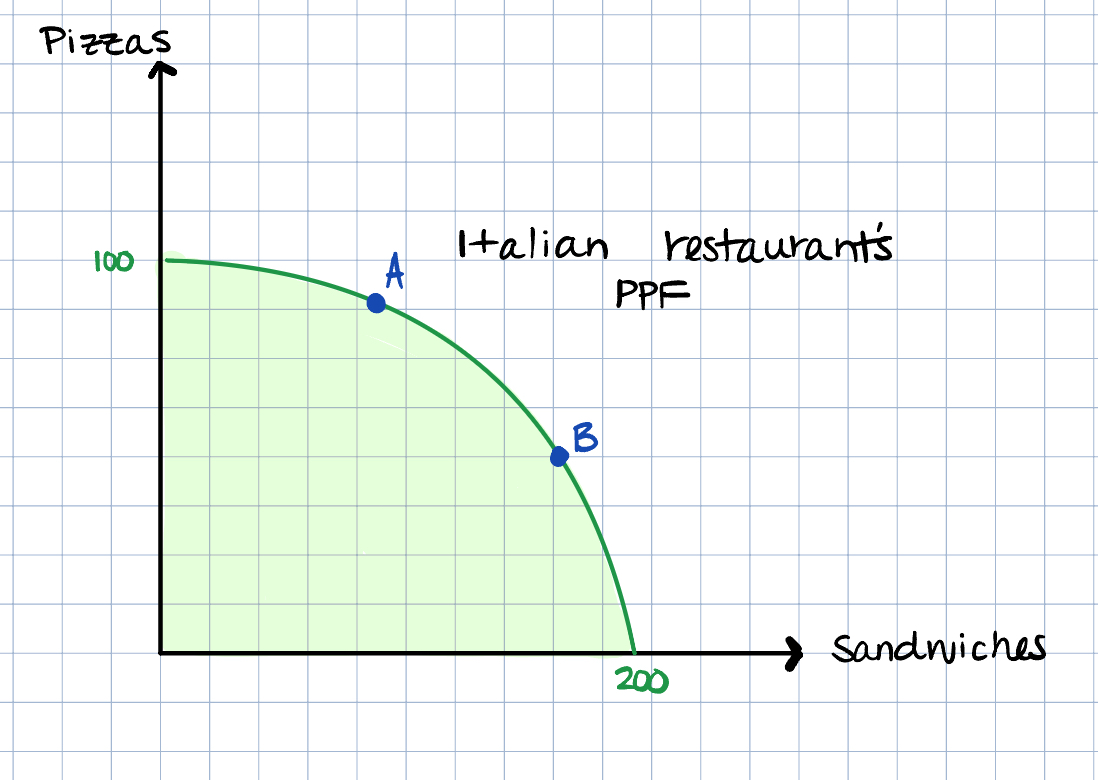
\includegraphics[width=.75\textwidth]{PPF.png}
    \caption{Production possibility frontier of the Italian restaurant}
    \label{fig:PPF}
\end{figure}

\medskip

\textbf{2.} It takes this concave shape because of technology constraints: we face diminishing returns for switching production from one technology to another. 

\medskip

Say we have a deli counter to make sandwiches, and a kitchen in the back to make pizzas. In addition we have a team of expert sandwich makers and a team of expert pizza chefs. Suppose we are using all of our resources (our space, our equipment, and our labor) to make only sandwiches. This means our ovens are being wasted, and our pizza artists are taking forever to produce one sandwich. When we start switching some of the pizza-making equipment over to doing what it is meant to do (making pizzas), we at first see really big benefits: sacrificing one sandwich in output, we might be able to make several pizzas. 

\medskip

This will quickly start to even out, as we get to the point where most of the sandwich workers/equipment are being used for sandwiches and most of the pizza workers/equipment are being used to make pizzas. If we continue switching our resources over to pizzas, we start to face the opposite problem: our sandwich experts are being made to make pizzas, and they're not doing a very good job. So the slope of the PPF grows very flat, since we can only get a small amount of pizzas for the amount of sandwiches we give up.

\medskip

\textbf{3.} Take any two points A and B and make up some numbers: suppose at A we produce 110 sandwiches and 80 pizzas, and at point B we produce 170 sandwiches and 50 pizzas. When we move from A to B, we are producing more sandwiches than before, and so we want to express the opportunity cost of that increased production in terms of pizzas we are no longer making:

$$
\text{opportunity cost } = 80 - 50 = 30 \text{ pizzas}
$$

We also might be interested in looking at the opportunity cost per sandwich. We can do this by adding the change in sandwiches produced into the denominator:

$$
\text{opportunity cost } = \dfrac{80 - 50 = 30 \text{ pizzas}}{170-110 = 60 \text{ sandwiches}} = 2 \text{ pizzas per sandwich}
$$

However, it is clear from the shape of the graph that it matters where we are on the PPF because the slope is not constant. To see this, check what the opportunity cost (on a per-unit basis) would be if we moved from producing \textit{only} pizzas to producing \textit{only} sandwiches. That would look like this:
$$
\text{opportunity cost } =  100 - 0 = 100 \text{ pizzas}
$$
or
$$
\text{opportunity cost } = \dfrac{100 - 0 = 100 \text{ pizzas}}{200-0 = 200 \text{ sandwiches}} = \frac{1}{2} \text{ pizzas per sandwich}
$$


\medskip

\textbf{4.} Things that might change the shape of the PPF over time will be related to the production process: a new type of pizza oven that is more efficient, a change in the cost of labor, or a new technique for making 10 sandwiches at one time are all examples of a change in the production process. Let's think about a specific example, and use it to distinguish a change in the \textit{shape} of the PPF.

\medskip

Suppose a new pizza oven makes us able to produce 50\% more pizzas than we were before, holding the input (workers, ingredients, etc.) fixed\footnote{This is a pretty magical pizza oven since we can make more pizza without using more ingredients.}. Instead of producing 100 pizzas when we are devoting all of our resources to pizzas, we can produce 150. However, nothing has changed for our ability to produce sandwiches, so we can still only produce 200 when we devote all of our resources to sandwiches. So the shape of our PPF has changed, illustrated in figure \ref{fig:PPFshape}. 

\begin{figure}
    \centering
    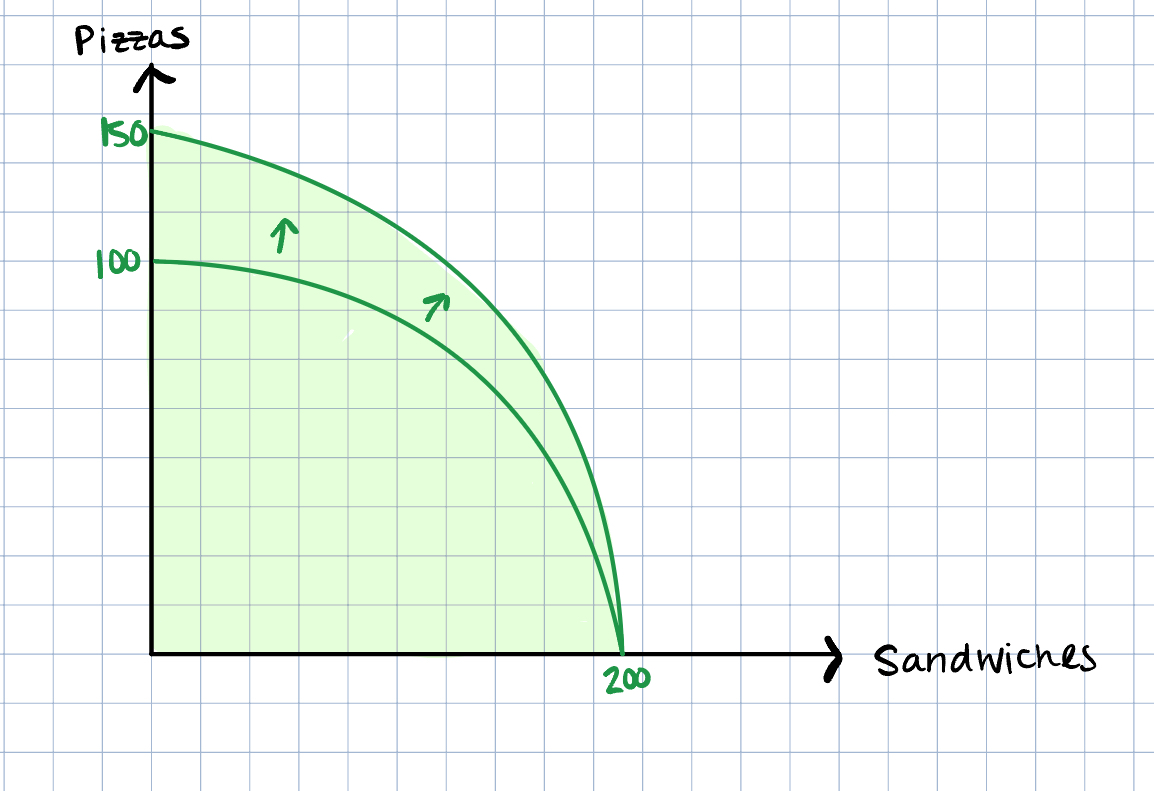
\includegraphics[width=.75\textwidth]{PPFshape.png}
    \caption{A change in the shape of the PPF}
    \label{fig:PPFshape}
\end{figure}

\medskip

Now suppose that we have a new investor, and he has given us double the resources (staff, space, equipment, ingredients, etc.). Also assume that we have ``constant returns to scale'' for each product --- this just means that twice the workers with twice the equipment can produce twice the pizzas. Now we haven't changed anything about the technology itself, so the tradeoff between making pizzas and making sandwiches is the same as before, we can just now make twice as many of them. This means that the \textit{shape} of our PPF is the same, it's just moved further out in a uniform way, as shown in figure \ref{fig:PPFshift}.

\begin{figure}
    \centering
    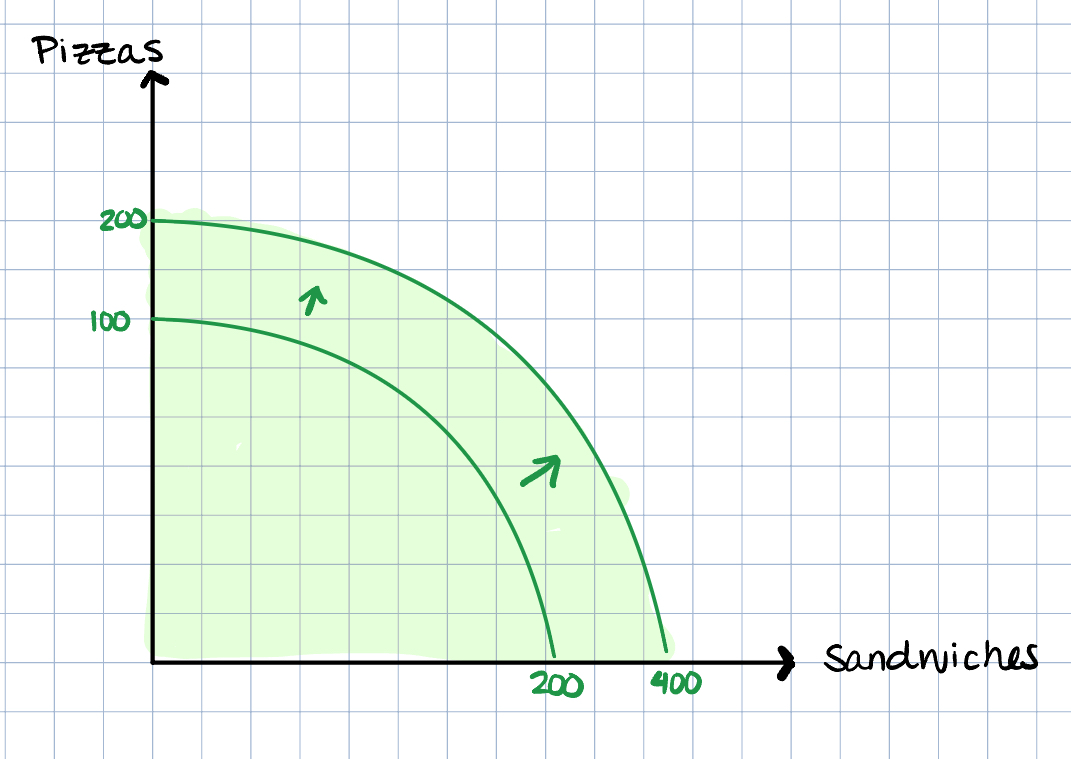
\includegraphics[width=.75\textwidth]{PPFshift.png}
    \caption{A shift in the PPF}
    \label{fig:PPFshift}
\end{figure}

\medskip

\subsection*{Question 3: CPF of a consumer}
Now suppose we are \textit{going} to the Italian restaurant with a group of friends, and we want to decide what to order. Pizzas are \$10, sandwiches are \$5, and we have \$100 to spend.
    \begin{enumerate}
        \item What will our consumption possibility frontier look like?
        \item What is the opportunity cost of a pizza? Does it matter where on the CPF we are?
        \item What will happen to the CPF if we have \$200 to spend?
        \item What will happen to the CPF if the price of sandwiches increases to \$10?
    \end{enumerate}

    \medskip

    \textbf{Answer:}

\textbf{1.} In this case, our CPF is just a straight line. Unlike with the PPF, there are no decreasing returns as we buy more sandwiches and fewer pizzas. The consumption set and consumption possibility frontier are shown in figure \ref{fig:CPF}. The whole set of possible consumption combinations of pizza and sandwiches is represented by the blue shaded region, while the consumption possibility frontier is the darker blue line.

\begin{figure}[H]
    \centering
    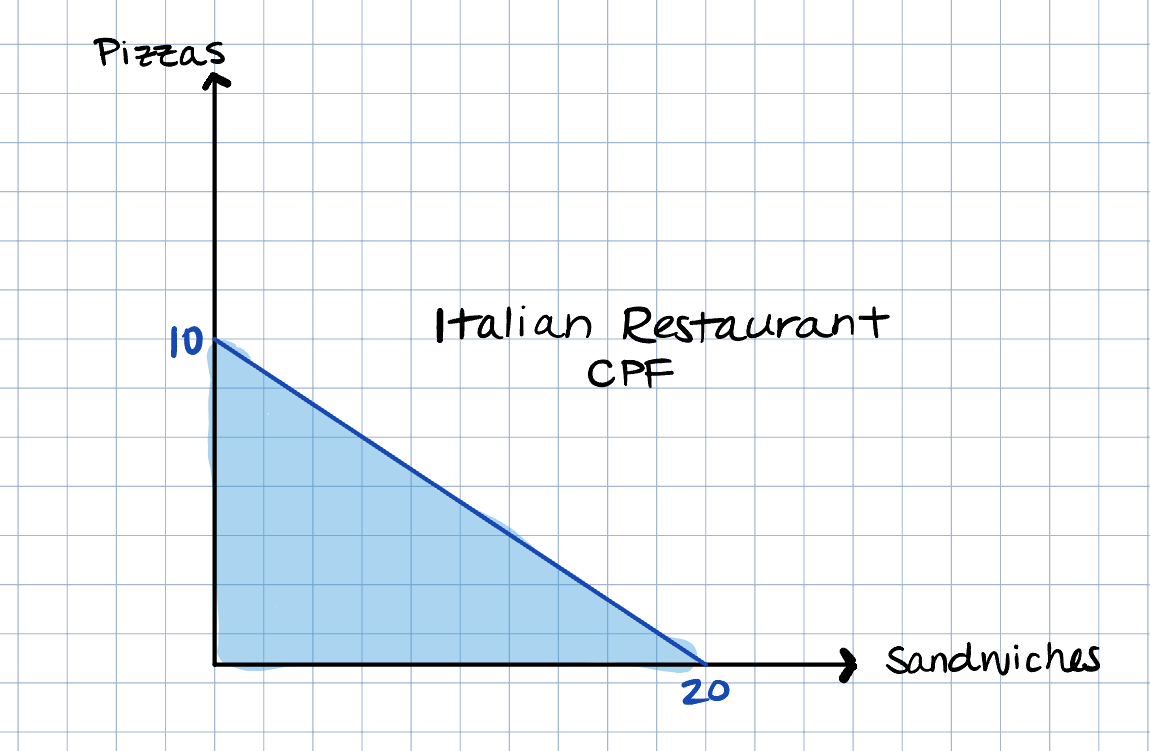
\includegraphics[width=.75\textwidth]{CPF.png}
    \caption{Consumption possibility frontier for Italian food}
    \label{fig:CPF}
\end{figure}

\textbf{2.} Since I provided specific numbers, we can actually draw the CPF (also called a budget line) and do some calculations. We have \$100 and pizzas cost \$10, so if we only buy pizzas, we can buy 10. Thus we put one point at 10 pizzas and 0 sandwiches. Alternatively, we can buy only sandwiches: since they are \$5, we can buy 20 of them if we buy no pizzas.

\medskip

We know from algebra that two points on a straight line are all that we need to calculate its slope:

$$
m = \dfrac{(y_2 - y_1)}{(x_2 - x_1)} = \dfrac{0 - 10}{20 - 0} = - \frac{1}{2}
$$

We can also see that the line intersects the $y$ (pizza) axis at 10. Recalling the formula for a line $y = mx + b$, where $m$ is the slope and $b$ is the y-intercept, we can describe the CPF with the equation:

$$
y = -\frac{1}{2}x + 10
$$

or alternatively

$$
\text{pizzas } = -\frac{1}{2} \text{ sandwiches } + 10
$$

To see this is true, just throw in one of our points and double-check that both sides agree.

\medskip

So, what is the opportunity cost of pizza? Since the slope is constant, it doesn't matter which points we use to test this out, and we may as well use the end points of the line. If we start off with 0 sandwiches and 10 pizzas, and move to 20 sandwiches and 0 pizzas, our opportunity cost is $\frac{10 \text{ pizzas}}{20 \text{ sandwiches}} = \frac{1}{2}$ pizzas per sandwich.

\medskip

\textbf{3.} With \$200 instead of \$100, we can now afford 20 pizzas and 0 sandwiches on the one end, or 40 sandwiches and 0 pizzas on the other. In other words, we have moved out our CPF and expanded the size of our possible consumption set. This is a shift in our CPF, but it does not change the shape of it (note that the slope is the same --- check this!). FIgure ~\ref{fig:CPFshift} depicts this shift in the CPF.

\begin{figure}[H]
    \centering
    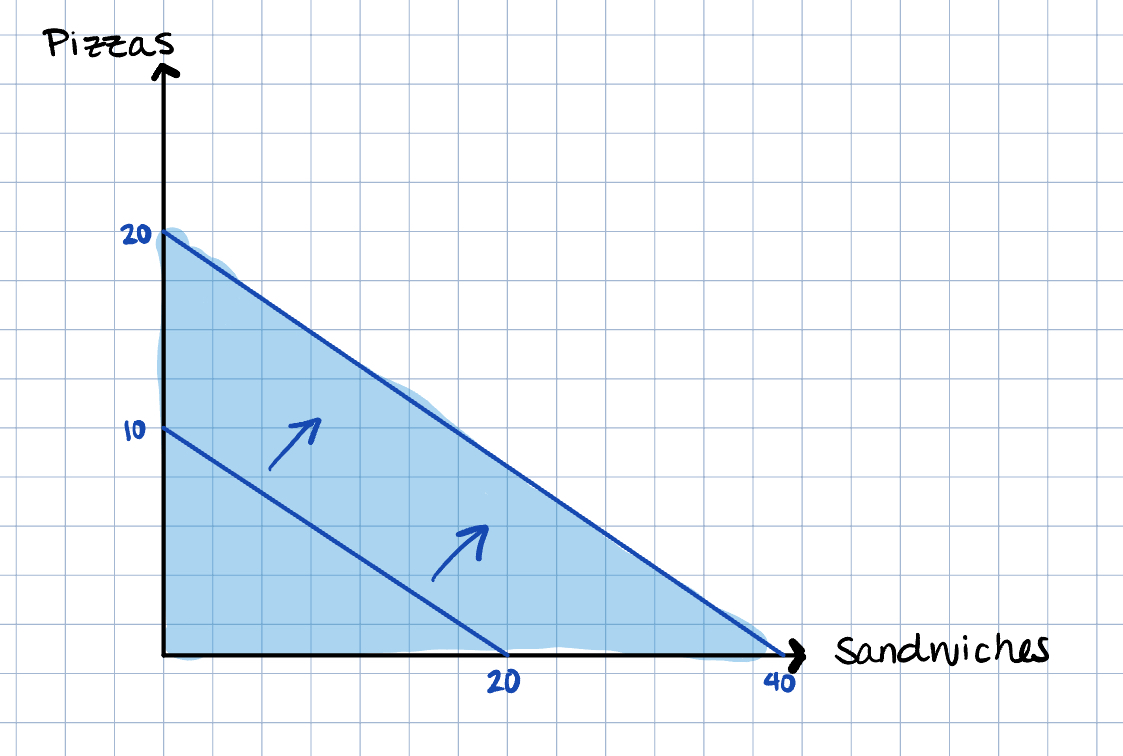
\includegraphics[width=.75\textwidth]{CPFshift.png}
    \caption{Consumption possibility frontier shift}
    \label{fig:CPFshift}
\end{figure}

\medskip

\textbf{4.} Return to only having \$100 to spend. While we can still afford 10 pizzas and 0 sandwiches, with sandwiches costing \$10 we now can only afford 10 sandwiches and 0 pizzas. This causes a pivot to the left of the x-axis intercept, and our entire consumption set has shrunk. This actually changes the \textit{shape} of the CPF, as opposed to the example in question 3. Figure~\ref{fig:CPFshape} depicts this shape change.

\begin{figure}[H]
    \centering
    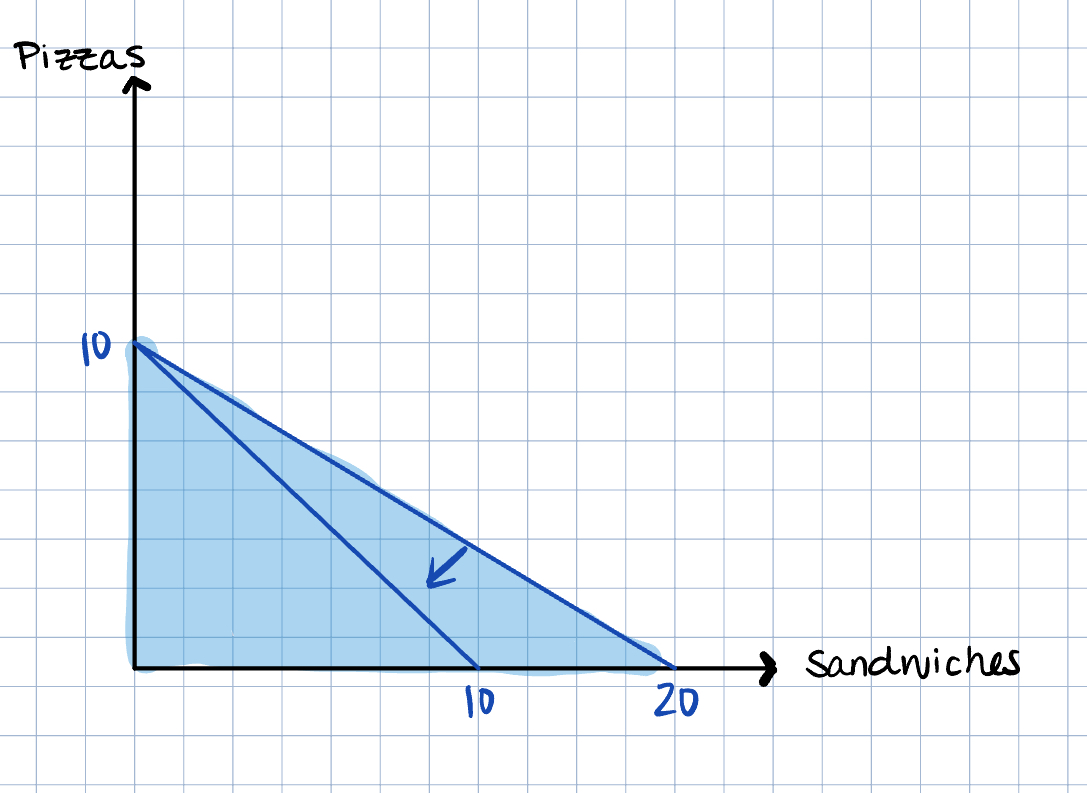
\includegraphics[width=.75\textwidth]{CPFshape.png}
    \caption{Consumption possibility frontier shape change}
    \label{fig:CPFshape}
\end{figure}

\subsection*{Question 4: Italian restaurant economy}
Suppose the entire economy consists of Italian restaurants: during half of the week we work in one, and during the other half we buy food from them.
\begin{enumerate}
    \item What does the circular-flow diagram look like?
    \item What is missing from our model?
\end{enumerate}

\medskip

\textbf{Answer:}

Your circular-flow diagram might look something like figure \ref{fig:CFD}.

\begin{figure}[H]
    \centering
    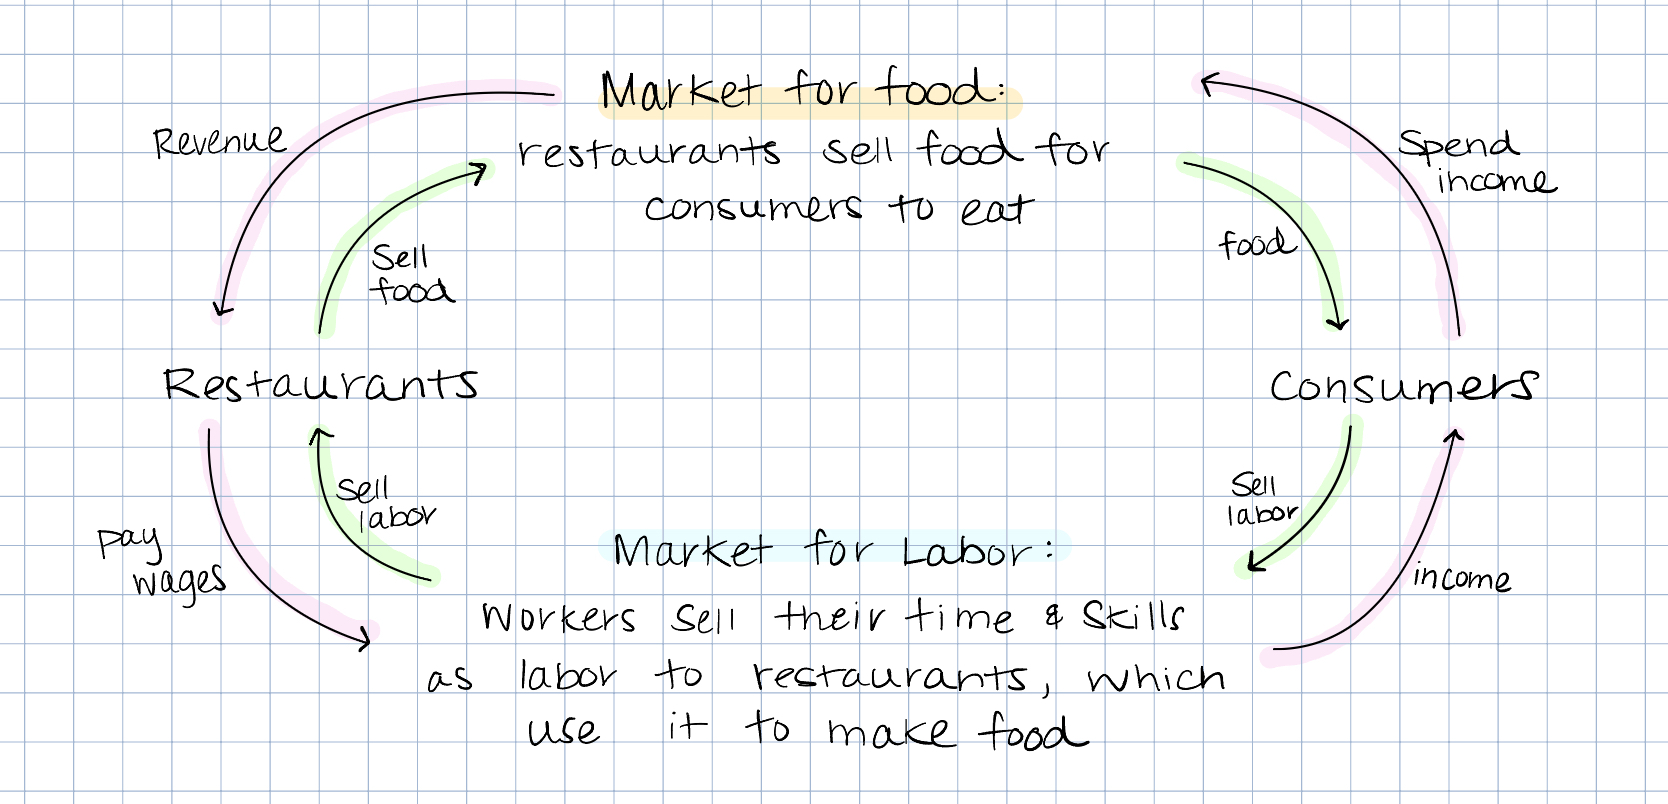
\includegraphics[width=\textwidth]{CFD.png}
    \caption{Circular-flow diagram of the Italian restaurant Economy}
    \label{fig:CFD}
\end{figure}

Of course this is an extremely simplified (``stylized'' in economics-talk) model of the economy, and there are plenty of things you could mention that are left out. One obvious example would be a public sector; perhaps workers and firms pay taxes to a government, which in turn provides services to them. Another example would be household savings and a financial sector.

\medskip

\subsection*{Question 5: Guiding Economic Policy}
Economists are often asked to guide economic policy...
\medskip
\begin{enumerate}
    \item What are positive and normative statements?
    \begin{enumerate}
        \item Can you give an example of each?
    \end{enumerate}
    \item Why might two economists make different suggestions?
    \item Why might a politician ignore an economist's suggestions?
\end{enumerate}

\medskip

\textbf{Answer:}

\begin{enumerate}
    \item A \textbf{positive} statement is one that is a fact and cannot be refuted. A \textbf{normative} statement is one of opinion and is not necessarily true.
\medskip
A quick and simple way to remember the meaning behind these two terms are as follows:
\begin{center}
    Positive statement:  \textit{You are \textbf{POSITIVE} the statement is true} \\
    Normative statement: \textit{This statement is \textbf{NORMALLY} true in my opinion}
\end{center}
This is how I remembered the meaning behind these two statements when I was taking this class! 
    \begin{enumerate}
        \item Example of a positive statement: We will celebrate 150 years of JHU in 2026. \\
        Example of a normative statement: We ought to do more to help the poor.
    \end{enumerate}
    \item Economists may have different hunches about the validity of conflicting economic theories, among other reasons.
    \item Political success relies on more than just economic efficiency.
\end{enumerate}


\end{document}


